\documentclass[svgnames,tikz]{standalone}
\usepackage{pgfmath}
\usetikzlibrary{positioning,arrows,calc,3d}

\tikzset{
  focus/.style args={#1 at #2}{
    insert path={
      %{ [white] (#2.north east) rectangle (#2.south west)}
      ($(#2.center)!#1!(#2.north east) $) rectangle ($(#2.center)!#1!(#2.south west) $)
    }
  },
  focusout/.style args={#1 at #2}{
    even odd rule,
    insert path={
      (#2.north east) rectangle (#2.south west)
      ($(#2.center)!#1!(#2.north east) $) rectangle ($(#2.center)!#1!(#2.south west) $)
    }
  },
  txt/.style={font=\Large\tt},
  img/.style={
     inner sep=2pt,
     draw,
     label/.append style={font=\small\tt},
  },
}


\begin{document}
\begin{tikzpicture}
\tikzset{every node/.style={node distance=5pt, font=\Huge}}

\node[txt] (p0) { zip( };

\node[img, yslant=.5] (p1) [right=1cm of p0.center] { 
\includegraphics[width=3cm]{../../images/lena_red.png} };

\node[txt] (p2) [right=4.2cm of p0.center] { , };

\node[img, yslant=.5] (p3) [right=5cm of p0.center] { 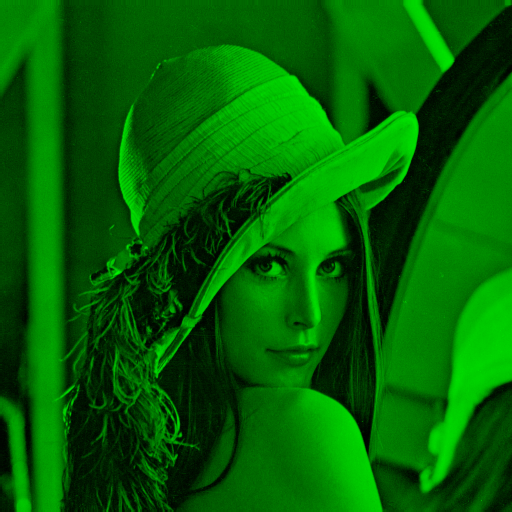
\includegraphics[width=3cm]{../../images/lena_green.png} };

\node[txt] (p4) [right=8.2cm of p0.center] { , };

\node[img, yslant=.5] (p5) [right=9cm of p0.center] { 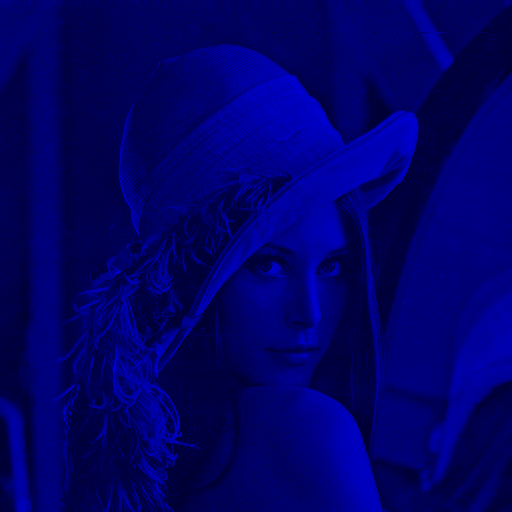
\includegraphics[width=3cm]{../../images/lena_blue.png} };

\node[txt] (p6) [right=12.4cm of p0.center] { ) $\rightarrow$ };

\begin{scope}[yscale=1, transform shape]
  \node[img, yslant=.5] (p7) [right=15.7cm of p0.center] { 
\includegraphics[width=3cm]{../../images/lena_red.png} };
  \node[img, xshift=1cm, yslant=.5] (p8) [right=15.7cm of p0.center] { 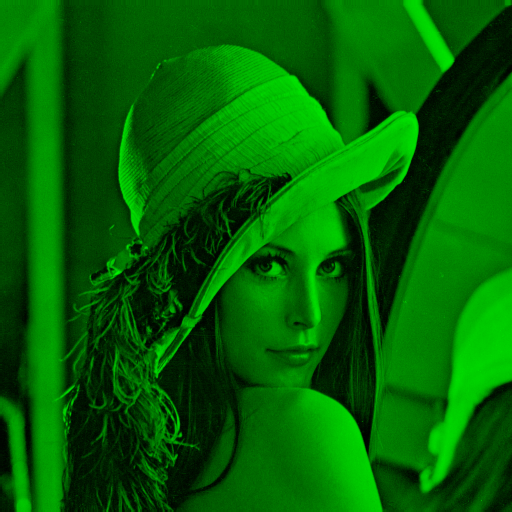
\includegraphics[width=3cm]{../../images/lena_green.png} };
  \node[img, xshift=2cm, yslant=.5] (p9) [right=15.7cm of p0.center] { 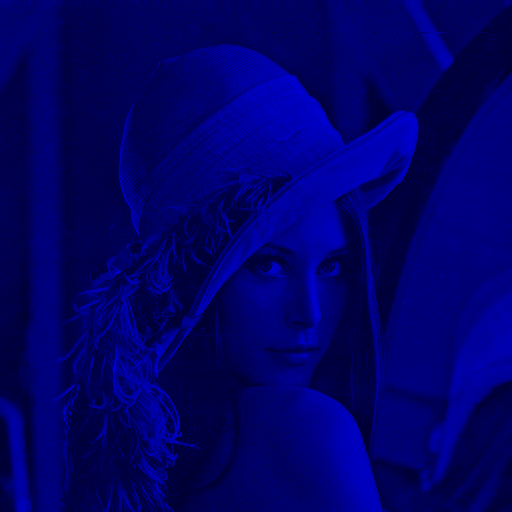
\includegraphics[width=3cm]{../../images/lena_blue.png} };
\end{scope}

\node[txt] (p10) [right=13.6cm of p0.center] { Image( };
\node[txt] (p11) [right=21.2cm of p0.center] { ) };

\end{tikzpicture}
\end{document}
